\documentclass{standalone}
%\usepackage[subpreambles=true]{standalone}
%\usepackage{xcolor}
\usepackage{latexcolors}
\usepackage{tikz}
\usetikzlibrary{positioning}
\usetikzlibrary {arrows.meta}
\begin{document}
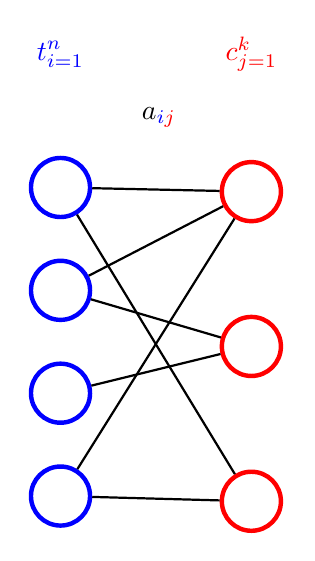
\begin{tikzpicture}

\def\labfont{\bfseries\normalsize}

%\node[font=\labfont,anchor=mid](A) at (1.25cm,-.75cm){$A(\textcolor{blue}{t},\textcolor{red}{c})$};
\node[font=\labfont,anchor=mid](A) at (1.25cm,-.75cm){$a_{\textcolor{blue}{i}\textcolor{red}{j}}$};



\node[font=\labfont,anchor=mid] (tags) at (0,0) {\textcolor{blue}{$t^n_{i=1}$}};

\node[font=\labfont,right=2cm of tags,anchor=mid]  (clouds) {\textcolor{red}{$c^k_{j=1}$}};

\node[anchor=mid,draw=blue,circle,  ultra thick, minimum size=.75cm, below=1cm of tags](T1){};
\node[anchor=mid,draw=blue, circle, ultra thick, minimum size=.75cm, below=.5cm of T1](T2) {};
\node[anchor=mid,draw=blue, circle, ultra thick, minimum size=.75cm, below=.5cm of T2](T3) {};
\node[anchor=mid,draw=blue, circle, ultra thick, minimum size=.75cm, below=.5cm of T3](T4) {};
\node[anchor=mid,draw=red, circle, ultra thick, minimum size=.75cm, below=1cm of clouds](C1) {};
\node[anchor=mid,draw=red, circle, ultra thick, minimum size=.75cm, below=1.16cm of C1](C2) {};
\node[anchor=mid,draw=red, circle, ultra thick, minimum size=.75cm, below=1.16cm of C2](C3) {};
%\node[anchor=mid,draw=red, circle, ultra thick, minimum size=.75cm, below=.4cm of C3](C4) {};



% \draw[thick,-Stealth] (C1) -- (T1);
% arrow if we need it
\draw[thick] (C1) -- (T1);
\draw[thick] (C1) -- (T2);
\draw[thick] (C1) -- (T4);
\draw[thick] (C2) -- (T2);
\draw[thick] (C2) -- (T3);
\draw[thick] (C3) -- (T1);
\draw[thick] (C3) -- (T4);
% \draw[thick,-Stealth] (C4) -- (T4);
\end{tikzpicture}
\end{document}